\documentclass[11pt, dvipsnames, handout]{beamer}
\newtoggle{full}
\settoggle{full}{true}

\newtoggle{covered}
\settoggle{covered}{false}

\newtoggle{presentable}
\settoggle{presentable}{false}

\newtoggle{dualscreen}
\settoggle{dualscreen}{false}

\usepackage{pgfplots}
%\pgfplotsset{compat = newest}

\usepackage{pgfpages}

\setbeamertemplate{note page}{\pagecolor{yellow!5}\vfill \insertnote \vfill}
\usepackage{collect}
\definecollection{notes}
\newcounter{notestaken}

\usepackage{xpatch}

\usepackage{ulem}

\usepackage[framemethod=tikz]{mdframed}

\usepackage{scalerel}
\usepackage{calc}

%\usepackage{enumitem}
\setlength\fboxsep{.2em}

\usepackage{graphicx} % Allows including images
\usepackage{booktabs} % Allows the use of \toprule, \midrule and \bottomrule in tables

\xpatchcmd{\itemize}
  {\def\makelabel}
  {\setlength{\itemsep}{0.65 em}\def\makelabel}
  {}
  {}


\xpatchcmd{\beamer@enum@}
  {\def\makelabel}
  {\setlength{\itemsep}{0.65 em}\def\makelabel}
  {}
  {}


%\makeatletter
%\renewcommand{\itemize}[1][]{%
%  \beamer@ifempty{#1}{}{\def\beamer@defaultospec{#1}}%
%  \ifnum \@itemdepth >2\relax\@toodeep\else
%    \advance\@itemdepth\@ne
%    \beamer@computepref\@itemdepth% sets \beameritemnestingprefix
%    \usebeamerfont{itemize/enumerate \beameritemnestingprefix body}%
%    \usebeamercolor[fg]{itemize/enumerate \beameritemnestingprefix body}%
%    \usebeamertemplate{itemize/enumerate \beameritemnestingprefix body begin}%
%    \list
%      {\usebeamertemplate{itemize \beameritemnestingprefix item}}
%      {%
%        \setlength\topsep{1em}%NEW
%        \setlength\partopsep{1em}%NEW
%        \setlength\itemsep{1em}%NEW
%        \def\makelabel##1{%
%          {%
%            \hss\llap{{%
%                \usebeamerfont*{itemize \beameritemnestingprefix item}%
%                \usebeamercolor[fg]{itemize \beameritemnestingprefix item}##1}}%
%          }%
%        }%
%      }
%  \fi%
%  \beamer@cramped%
%  \raggedright%
%  \beamer@firstlineitemizeunskip%
%}
%
%
%
%
%
%\makeatother

%\setlist[beamer@enum@]{topsep=1 em}
%\let\origcheckmark\checkmark %screw you dingbat
%\let\checkmark\undefined %screw you dingbat
%\usepackage{dingbat} 
%\let\checkmark\origcheckmark %screw you dingbat






%\usepackage{fontawesome}

\usepackage{mathtools}
\usepackage{etoolbox, calculator}

\usepackage{xcolor}
\usepackage{tikz}
\usetikzlibrary{arrows.meta}
\usetikzlibrary{calc}
\usepackage[nomessages]{fp}
\usepackage{transparent}
\usepackage{accsupp}
%\usepackage{color, xcolor}

%colorblind-friendly palette
%\definecolor{dblue}{RGB}{51,34,136}
\definecolor{lblue}{RGB}{136,204,238}
%\definecolor{green}{RGB}{17,119,51}
\definecolor{tan}{RGB}{221,204,119}
%\definecolor{mauve}{RGB}{204,102,119}

\usepackage{tcolorbox}



\usepackage{xifthen}
\usepackage{nicefrac}
\usepackage{amsmath}
\usepackage{amsthm}
\usepackage{amssymb}
\theoremstyle{definition}
\newtheorem*{define}{Definition}
\newtheorem*{recall}{Recall}


\DeclareMathOperator{\tr}{tr}

\usepackage{multicol}
%\setlength{\columnsep}{1cm}

\usepackage{tablists, amsmath,vwcol, cancel, polynom}
\usetikzlibrary{shapes, patterns, decorations.shapes}
%\usepackage{tikzpeople}
\tikzstyle{vertex}=[shape=circle, minimum size=2mm, inner sep=0, fill]
\tikzstyle{opendot}=[shape=circle, minimum size=2mm, inner sep=0, fill=white, draw]

% common math quick commands
\newcommand{\nicedd}[2]{\nicefrac{\text{d}#1}{\text{d}#2}}
\newcommand{\dd}[2]{\dfrac{\text{d}#1}{\text{d}#2}}
\newcommand{\pd}[2]{\dfrac{\partial #1}{\partial#2}}
\renewcommand{\d}[1]{\text{d}#1}
\newcommand{\ddn}[3]{\dfrac{\text{d}^{#3}#1}{\text{d}#2^{#3}}}
\newcommand{\pdn}[3]{\dfrac{\partial^{#3}#1}{\partial#2^{#3}}}
\newcommand{\p}[0]{^{\prime}}
\newcommand{\pp}[0]{^{\prime\prime}}
\newcommand{\op}[2][\text{L}]{#1 \left[ #2 \right]}

\newcommand{\lap}[1]{\mathcal{L}\left\{#1\right\}}
\newcommand{\lapinv}[1]{\mathcal{L}^{-1}\left\{#1\right\}}
\newcommand{\lapint}[1]{\int_0^\infty e^{-st}#1dt}
\newcommand{\evalat}[2]{\Big|_{#1}^{#2}}

\newcommand{\paren}[1]{ \left( #1 \right)}

\newcommand{\haxis}[4][\normcolor]{\draw[#1, <->] (-#2,0)--(#3,0) node[right]{$#4$}; }

\newcommand{\circled}[1]{\raisebox{.5pt}{\textcircled{\raisebox{-.9pt} {#1}}}}
\newcommand{\axis}[4]{\draw[\normcolor, <->] (-#1,0)--(#2,0) 
node[right]{$x$};
\draw[help lines, <->] (0,-#3)--(0,#4) node[above]{$y$};}

\newcommand{\laxis}[6]{\draw[<->] (-#1,0)--(#2,0) 
node[right]{$#5$};
\draw[ <->] (0,-#3)--(0,#4) node[above]{$#6$};}
\newcommand{\xcoord}[2]{
	\draw (#1,.2)--(#1,-.2) node[below]{$#2$};}
\newcommand{\textnode}[3]{
	\draw (#1,#2) node[below]{$#3$};}
	
\newcommand{\nxcoord}[2]{
	\draw (#1,-.2)--(#1,.2) node[above]{$#2$};}
\newcommand{\ycoord}[2]{
	\draw (.2,#1)--(-.2,#1) node[left]{$#2$};}
\newcommand{\nycoord}[2]{
	\draw (-.2,#1)--(.2,#1) node[right]{$#2$};}
\newcommand{\dlim}{\displaystyle\lim}
\newcommand{\dlimx}[1]{\displaystyle\lim_{x \rightarrow #1}}
\newcommand{\stickfig}[2]{
	\draw (#1,#2) arc(-90:270:2mm);
	\draw (#1,#2)--(#1,#2-.5) (#1-.25,#2-.75)--(#1,#2-.5)--(#1+.25,#2-.75) (#1-.2,#2-.2)--(#1+.2,#2-.2);}	

%\newcounter{example}
%\setcounter{example}{1}
%\newcounter{preFrameExample}
%\AtBeginEnvironment{frame}{\setcounter{preFrameExample}{\value{example}}}
%\newcommand{\ex}[1]{
%	 \setcounter{example}{\value{preFrameExample}}
%	 \textcolor{green}{\small\fbox{Example \arabic{example}: #1}}\\[8pt]
%	\stepcounter{example}}
%\newcommand{\exans}[1]{
%	\SUBTRACT{\value{preFrameExample}}{1}{\n}
%	 \textcolor{green}{\small\fbox{Solution \n: #1}}\\[8pt]}
\mode<presentation> {

% The Beamer class comes with a number of default slide themes
% which change the colors and layouts of slides. Below this is a list
% of all the themes, uncomment each in turn to see what they look like.


\usetheme{CambridgeUS}
\usecolortheme[named=black]{structure}


\newcommand{\studentcolor}[0]{ForestGreen}
\newcommand{\normcolor}[0]{NavyBlue}
\newcommand{\alertcolor}{Red}

\setbeamercolor{normal text}{fg=\normcolor}
\setbeamercolor{frametitle}{fg=\normcolor}
\setbeamercolor{section in head/foot}{fg=Black, bg=Gray!20}
\setbeamercolor{subsection in head/foot}{fg=Green!70!Black, bg=Gray!10}
\setbeamercolor{alerted text}{fg=\alertcolor}
\setbeamerfont{alerted text}{series=\bf}
\setbeamertemplate{enumerate items}[default]
\setbeamercolor{enumerate item}{fg=\normcolor}

\setbeamertemplate{footline} % To remove the footer line in all slides uncomment this line
%\setbeamertemplate{footline}[page number] % To replace the footer line in all slides with a simple slide count uncomment this line

\setbeamertemplate{navigation symbols}{} % To remove the navigation symbols from the bottom of all slides uncomment this line
}

\newcommand{\alertbox}[1]{\tcbox[on line, colframe=\alertcolor, colback=White, left=2pt,right=2pt,top=2pt,bottom=2pt]{\usebeamercolor*{normal text}#1}}


\newcommand{\startstu}{\setbeamercolor{normal text}{fg=\studentcolor}\usebeamercolor*{normal text}\setbeamercolor{enumerate item}{fg=\studentcolor}\usebeamercolor*{enumerate item}}
\newcommand{\stopstu}{\setbeamercolor{normal text}{fg=\normcolor}\usebeamercolor*{normal text}\setbeamercolor{enumerate item}{fg=\normcolor}\usebeamercolor*{enumerate item}}

\newcommand{\takenote}[1]{ \begin{collect}{notes}{}{}{}{}  #1  \end{collect}  \addtocounter{notestaken}{1}} %\ifthenelse{\value{notestaken}>0}{\hrulefill\\}{}

\makeatletter
\newcommand{\cover}{\alt{\beamer@makecovered}{\beamer@fakeinvisible}}
\newcommand{\ucover}[1]{\iftoggle{full}{}{\beamer@endcovered} \stopstu #1\startstu \iftoggle{full}{}{\beamer@startcovered} }
%\newcommand{\ucover}[1]{\beamer@endcovered \stopstu #1\startstu \beamer@startcovered }
\makeatother

\newcommand{\skippause}{ \addtocounter{beamerpauses}{-1}}
\newcommand{\blockpres}{ \skippause \pause }

\newcommand{\studentify}[1]{\startstu #1  \stopstu }
\newcommand{\student}[1]{\iftoggle{full}{ \pause  \studentify{#1} }{\iftoggle{covered}{\studentify{#1}}{\cover{  #1 }}}}
\newcommand{\cstudent}[1]{\student{\begin{center} #1 \end{center}}}
\newcommand{\fullonly}[1]{\iftoggle{full}{ #1}{}}
\newcommand{\presentonly}[1]{\iftoggle{presentable}{ #1}{}}

\usepackage{xparse}
\usepackage{xifthen}

% shortcuts for commonly-used presentation elements
%\NewDocumentCommand{\slide}{o m}
% {\IfValueTF{#1}{\begin{frame}[t]{#1}}{\begin{frame}[t]} #2 \end{frame}}

\newtoggle{iscovered}

\newcommand{\slide}[2][]{%
%\setcounter{notestaken}{0}
\takenote{#2} 
%\ifthenelse{\equal{#1}{}}{\begin{frame}[t]}{\begin{frame}[t]{#1}} #2 \ifthenelse{\value{notestaken}>0}{ \note{\includecollection{notes}}}{} \end{frame}%
\ifthenelse{\equal{#1}{}}{\begin{frame}[t]}{\begin{frame}[t]{#1}} #2 \iftoggle{covered}{\settoggle{iscovered}{true}}{\settoggle{iscovered}{false}}  \note{ \iftoggle{iscovered}{}{\settoggle{covered}{true}} #2 \iftoggle{iscovered}{}{\settoggle{covered}{false}} } \end{frame}%
%\setcounter{notestaken}{0}
}
\newcommand{\defn}[2][]{%
 \setcounter{listcounter}{0}%
\ifthenelse{\equal{#1}{}}{\begin{block}{Definition}}{\begin{block}{#1 :}}%
 #2 \vspace{0.25em} \ifthenelse{\value{listcounter}>0}{\skippause}{} \pause \end{block}%
}



\newcommand{\arr}[2]{\begin{array}{#1}#2\end{array}}
\newcommand{\mat}[2]{\left[\arr{#1}{#2}\right]}
\newcommand{\carray}[1]{\arr{c}{#1}}
\newcommand{\larray}[1]{\arr{l}{#1}}
\newcommand{\rarray}[1]{\arr{r}{#1}}
\newcommand{\colvec}[1]{\mat{c}{#1}}

\newcommand{\itmz}[1]{\addtocounter{listcounter}{1} \begin{itemize}#1 \end{itemize} }
\newcommand{\subitem}[1]{\addtocounter{listcounter}{1} \begin{itemize} \item #1 \end{itemize}}
%
\newcommand{\enum}[1]{\addtocounter{listcounter}{1} \begin{enumerate} #1  \end{enumerate}  }


\newcommand{\algnlbl}[1]{\begin{align}#1  \end{align}} 
\newcommand{\algn}[1]{\begin{align*}#1  \end{align*}} 
\newcommand{\lgn}[1]{ \action<+->{#1} }
\newcommand{\slgn}[1]{\iftoggle{full}{\action<+->{ \startstu #1 \stopstu}}{ \cover{ #1 } } \takenote{$#1$}}

\newcommand{\chckmrk}{\alert{\checkmark}}

\usepackage{pifont}
\newcommand{\xmark}{\alert{\text{\large \ding{55}}}}

\newcommand{\return}[0]{\raisebox{.5ex}{\rotatebox[origin=c]{180}{$\Lsh$}}}
\usepackage{pbox}
%\newcommand{\ex}[1]{\rotatebox[origin=c]{10}{\uline{ex}}:$\;$\pbox[t][][b]{0.9\linewidth}{#1}}
\newcommand{\ex}[1]{\uline{ex}:$\;$\pbox[t][][t]{0.9\linewidth}{#1}}
\newcommand{\eg}[1]{e.g.,$\;$\pbox[t][][t]{0.9\linewidth}{#1}}
\newcommand{\tikzplot}[8][]{%
\begin{tikzpicture}

\begin{scope}[]%
\clip(-#2,-#4) rectangle (#3,#5);%
#8%
\end{scope}%
\laxis{#2}{#3}{#4}{#5}{#6}{#7}%
#1
\end{tikzpicture}%
}


\newcommand{\cancelslide}[1]{%
\begingroup%
\setbeamertemplate{background canvas}{%
\begin{tikzpicture}[remember picture,overlay]%
\draw[line width=2pt,red!60!black] %
  (current page.north west) -- (current page.south east);%
\draw[line width=2pt,red!60!black] %
  (current page.south west) -- (current page.north east);%
\end{tikzpicture}}%
#1%
\endgroup%
}
\renewcommand{\CancelColor}{\color{red}}
\newcommand{\twocols}[3][0.5]{\begin{columns}\begin{column}{#1\textwidth}#2\end{column}\hspace{1em}\vrule{}\hspace{1em}\begin{column}{#1\textwidth}#3\end{column}\end{columns}}

\newcommand{\twomini}[5][1]{\calculatespace \begin{minipage}[t]{\columnwidth}\begin{minipage}[][#1\contentheight][t]{#2\columnwidth}#4\end{minipage}\hfill\begin{minipage}[][#1\contentheight][t]{#3\columnwidth}#5\end{minipage}\end{minipage}}

\newcommand{\threemini}[7][1]{\calculatespace \begin{minipage}[t]{\columnwidth}\begin{minipage}[][#1\contentheight][t]{#2\columnwidth}#5\end{minipage}\hfill\begin{minipage}[][#1\contentheight][t]{#4\columnwidth}#6\end{minipage}\hfill\begin{minipage}[][#1\contentheight][t]{#3\columnwidth}#7\end{minipage}\end{minipage}}


\newcounter{listcounter}
\setcounter{listcounter}{0}



\newif\ifsidebartheme
\sidebarthemetrue

\newdimen\contentheight
\newdimen\contentwidth
\newdimen\contentleft
\newdimen\contentbottom
\makeatletter
\newcommand*{\calculatespace}{%
\contentheight=\paperheight%
\ifx\beamer@frametitle\@empty%
    \setbox\@tempboxa=\box\voidb@x%
  \else%
    \setbox\@tempboxa=\vbox{%
      \vbox{}%
      {\parskip0pt\usebeamertemplate***{frametitle}}%
    }%
    \ifsidebartheme%
      \advance\contentheight by-1em%
    \fi%
  \fi%
\advance\contentheight by-\ht\@tempboxa%
\advance\contentheight by-\dp\@tempboxa%
\advance\contentheight by-\beamer@frametopskip%
\ifbeamer@plainframe%
\contentbottom=0pt%
\else%
\advance\contentheight by-\headheight%
\advance\contentheight by\headdp%
\advance\contentheight by-\footheight%
\advance\contentheight by4pt%
\contentbottom=\footheight%
\advance\contentbottom by-4pt%
\fi%
\contentwidth=\paperwidth%
\ifbeamer@plainframe%
\contentleft=0pt%
\else%
\advance\contentwidth by-\beamer@rightsidebar%
\advance\contentwidth by-\beamer@leftsidebar\relax%
\contentleft=\beamer@leftsidebar%
\fi%
}
\makeatother



\iftoggle{dualscreen}{\setbeameroption{show notes on second screen=right}}{}
\usetikzlibrary{arrows}

\begin{document}
\section{Lecture 16}
\subsection{Preamble}
\settoggle{covered}{true}

\slide[\begin{minipage}{0.7\textwidth}Intro to Linear Systems:  Skydiving\end{minipage}\begin{minipage}{0.3\textwidth}{\hspace{5.25em}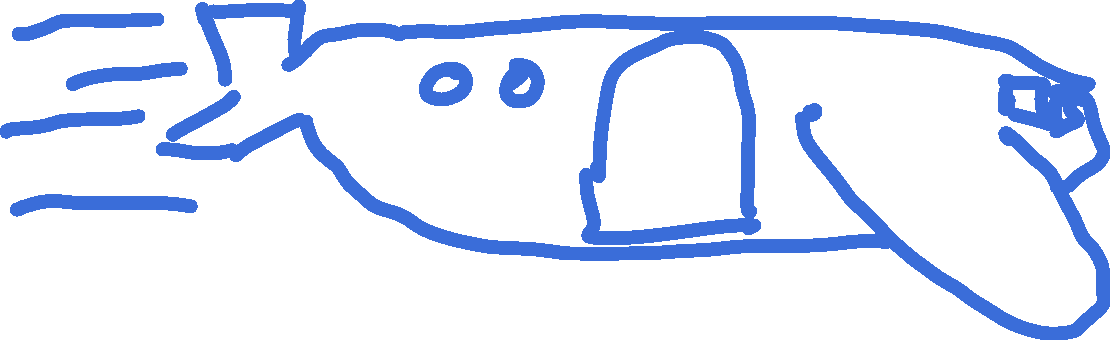
\includegraphics[height=.75cm]{images/airplane.pdf}}\end{minipage}]{  \begin{minipage}{0.6\textwidth} \vspace{-2em} Newton's 2$^{\text{nd}}$ Law: \end{minipage} \begin{minipage}{0.2\textwidth}\centerline{ 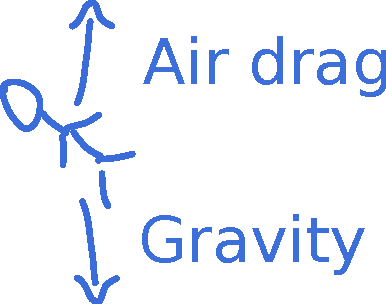
\includegraphics[width=2cm]{images/skydiver_solo.pdf}} \end{minipage} \hfill \vspace{-2em}\algn{ &ma = F(t)  = -mg - \mu v \intertext{noting that $a=x''$ and $v=x'$, we can rewrite this as}
 & \left. x'' + \frac{\mu}{m} x' = -g \quad  \right\} \text{2$^{nd}$ order ODE, one unknown function}}
\student{
or equivalently, \algn{  & \left. \begin{array}{c l}   x' &=v \\v' &= - \frac{\mu}{m} v-g\end{array}\right\} \text{1$^{st}$ order ODEs, two unknown functions}}
\vfill
Q: How do we find two unknown functions simultaneously?
}

}%end sldie



\slide[Linear Systems of DEs: Matrix Notation]{

\[ \text{$x\rightarrow x_1$, $v\rightarrow x_2$} \quad  \Rightarrow \quad \begin{array}{c l}  x_1' &=x_2\\x_2' &= - \frac{\mu}{m} x_2-g \end{array}\]
\student{
Using matrix notation:
\algn{ \dd{}{t}\mat{c}{x_1\\ x_2}  &= \mat{cc}{0&1\\0&-\frac{\mu}{m} }\mat{c}{x_1\\x_2} +\mat{c}{0\\g}\\\\
&=\mathbf{A} \vec{x} + \text{constant vector}
}
\vfill}

}

\slide[Linear Systems of DEs: Matrix Notation]{

General Linear System IVP:\[\dd{}{t}\vec{x} = \mathbf{A}(t) \vec{x} +\vec{f}(t) \quad\text{with} \quad \vec{x}(t_0)=\vec{x}_0\]
where $\mathbf{A}$ is an $n\times n$ matrix, and both $\vec{x}$ and $\vec{f}$ are $n\times1$ column vectors.
\vfill
\student{
Operator Form:
\algn{\dd{}{t}\vec{x} - \mathbf{A}(t) \vec{x}& = \vec{f}(t)\quad\text{with} \quad  \vec{x}(t_0)=\vec{x}_0\\
\op{\vec{x}} &= \vec{f}(t) }\vfill
\centerline{$\vec{f}(t)=\vec{0} \qquad \Rightarrow \qquad $homogeneous system}
}

}

\subsection{Converting between representations}
\slide[Equivalence of problems]{
For every $n^{th}$ order linear ODE, there is a corresponding system of $n$ 1$^{st}$ order linear ODEs.\vfill
\student{
\[a_n(t)x^{(n)}(t)+a_{n-1}(t)x^{(n-1)}(t) + \dots + a_0(t)x(t) = h(t)\]
can be expressed as 
\[\dd{}{t}\vec{x} = \mathbf{A}(t) \vec{x} +\vec{f}(t)\]
with \[\vec{x}(t)=\mat{c}{x\\x\p \\ \vdots \\ x^{(n-1)}}\]
}
}

\slide{
\ex{Rewrite $x'''+x'+x = t^2$ in the form $\dd{}{t}\vec{x} = \mathbf{A}\vec{x} + \vec{f}(t)$}\vfill
\student{\algn{\vec{x}&=\mat{c}{x_1\\x_2\\x_3} \quad \carray{x_1=x\\ x_2=x\p\\x_3=x\pp} \qquad\qquad \dd{}{t}\vec{x} =\mat{c}{x\p\\x\pp\\x'''} =  \mathbf{A}\vec{x} + \vec{f}(t)\\
x\p&=x_2\\
x\pp&=x_3\\
x'''&=-x -x\p+t^2\\
&=-x_1-x_2+t^2\\\\
 \dd{}{t}\vec{x}&=\mat{c}{x_1'\\x_2'\\x_3'} =\mat{c}{x\p\\x\pp\\x'''} = \underbrace{ \mat{ccc}{0&1&0\\0&0&1\\-1&-1&0}}_{\mathbf{A}} \mat{c}{x_1\\x_2\\x_3} \ + \underbrace{ \mat{c}{0\\0\\t^2}}_{\vec{f}}\\
}
}
}


\subsection{Finding solutions}

\slide[Skydiving: Homogeneous Solutions ]{
Suppose we want to solve $v\pp+\frac{\mu}{m}v\p=0$
\student{Guess $v(t)=e^{rt}$
\algn{r^2+\frac{\mu}{m}r &=0 &
r\left(r+\frac{\mu}{m}\right) &=0 \\ &r=0, -\frac{\mu}{m} 
&v(t) &= c_1+c_2e^{ -\frac{\mu}{m}t}\\
&&=c_1y_1(t) + c_2y_2(t)
}\vfill
What about for the vector expression?\vfill
\centerline{two LI homogeneous solutions $\quad \rightarrow \quad $ two LI vectors}\vfill
\algn{\vec{x}(t)  &=c_1 \mat{c}{1\\0} +c_2 e^{-\frac{\mu}{m} t} \mat{c}{1 \\ -\frac{\mu}{m}}\\\\
&=c_1\vec{x}_1(t) \;\;\;+\quad c_2\vec{x}_2(t) }
}
}




\slide[Homogeneous Problem and Superposition]{\vspace{-1em}
Suppose $\vec{x}_1(t), \;\vec{x}_2(t),\;\dots, \;\vec{x}_k(t)$ all solve the homogeneous problem \[\dd{}{t}\vec{x} = \mathbf{A}(t) \vec{x} \]\vfill
Then \[\vec{x}(t) = c_1\vec{x}_1(t)+c_2\vec{x}_2(t)+\dots+c_k\vec{x}_k(t)\]
also solves the same homogeneous problem.
\vfill
\student{
\algn{\dd{}{t}\vec{x} &= \sum_{i=1}^nc_i\dd{}{t}\vec{x}_i= \sum_{i=1}^nc_i \mathbf{A}(t) \vec{x}_i \\& =  \mathbf{A}(t)  \sum_{i=1}^nc_i\vec{x}_i \\
&=\mathbf{A}(t)\vec{x}(t)}
}
}
\settoggle{covered}{false}

\slide[Homogeneous Problem and Superposition]{\vspace{-1em}
Suppose $\vec{x}_1(t), \;\vec{x}_2(t),\;\dots, \;\vec{x}_k(t)$ all solve the homogeneous problem \[\dd{}{t}\vec{x} = \mathbf{A}(t) \vec{x} \]
\vspace{-2em}

Then the set of solutions \[ \left\{\vec{x}_1(t), \vec{x}_2(t), \dots,\vec{x}_k(t)\right\}\]
form a vector space $V$.
\vfill
\student{
Since we are using ``standard'' addition/multiplication we only need to check 2 properties\vfill
\enum{
\item Additive Closure\[\vec{x}_i+\vec{x}_j \in V \quad \checkmark \]
\item Scalar Closure:\\
For any constant c
\[c \vec{x}_j \in V \quad \checkmark \]
}
}
}

\slide[Homogeneous Problem and Superposition]{\vspace{-1em}
Suppose $\vec{x}_1(t), \;\vec{x}_2(t),\;\dots, \;\vec{x}_k(t)$ all solve the homogeneous problem \[\dd{}{t}\vec{x} = \mathbf{A}(t) \vec{x} \]
\vspace{-2em}

Then the set of solutions \[ \left\{\vec{x}_1(t), \vec{x}_2(t), \dots,\vec{x}_k(t)\right\}\]
form a vector space $V$.\vfill
\hrule
\vspace{.5em}
If $\mathbf{A}$ is $n\times n$, and we can find $n$ linearly independent solution vectors (i.e., $k=n$), then we have a solution basis. 
\vfill
That is, \uline{any} solution $\vec{x}(t)$ can be written as 
\student{\[\vec{x}(t) = c_1\vec{x}_1(t)+c_2\vec{x}_2(t)+\dots+c_n\vec{x}_n(t)\]}\small
See DiffyQs Appendixes A.4 \& A.5 for review of vector spaces and bases.
}


\slide[Finding the solution vectors $\vec{x}_i$]{
Given
\[\dd{}{t}\vec{x} = \mathbf{A} \vec{x},\]
we want to find one of its solution vectors.\vfill
\student{
For a scalar equation, if we have $y\p=ay$ then we know the solution is $y=ce^{at}$.
\vfill
Lets guess $\vec{x}(t)=e^{\lambda t}\vec{v}$, and plug it into the ODE
\algn{\lambda e^{\lambda t} \vec{v} &=  \mathbf{A} e^{\lambda t} \vec{v}\\
\lambda \vec{v} &= \mathbf{A} \vec{v}}
\vfill
$\vec{v}$ is an eigenvector of $\mathbf{A}$, and $\lambda$ is its associated eigenvalue.
}
}

\slide[Eigenvectors/Eigenvalues]{


\itmz{\item A $n \times n$ matrix has $n$ eigenvalues and eigenvectors \subitem{except in some special cases}
}\vfill
\student{
Ignoring those special cases for now, we can write any homogeneous solution as

\[\vec{x}(t) = c_1 e^{\lambda_1t}\vec{v}_1+c_2e^{\lambda_2 t}\vec{v}_2+\dots+c_ne^{\lambda_n t}\vec{v}_n\]
where $\vec{v}_i$ is the eigenvector associated with the eigenvalue $\lambda_i$.
\vfill

}\vspace{3em}
See DiffyQs \S 3.7 for details on those special cases.
}

\slide[Eigenvectors/Eigenvalues]{


\itmz{\item A $n \times n$ matrix has $n$ eigenvalues and eigenvectors \subitem{except in some special cases}
}\vfill
We want to find values $\lambda$ such that for some non-zero $\vec{v}$\[\mathbf{A}\vec{v} = \lambda \vec{v}\]
\student{
Rearrange as
\[(\mathbf{A} - \lambda \mathbf{I}) \vec{v} = \vec{0}\]
If $(\mathbf{A} - \lambda \mathbf{I})^{-1}$ exists, then \[\vec{v} =(\mathbf{A} - \lambda \mathbf{I})^{-1} \vec{0} = \vec{0} \]
So we need 
 \[\det(\mathbf{A} - \lambda \mathbf{I}) = 0\]

}\vspace{3em}
See DiffyQs \S A.6 for a review of determinants
}


\slide[Eigenvectors/Eigenvalues]{
\itmz{\item A $n \times n$ matrix has $n$ eigenvalues and eigenvectors \subitem{except in some special cases}
\item The eigenvalues are obtained from the roots of the characteristic polynomial obtained from   \[\det(\mathbf{A} - \lambda \mathbf{I}) = 0,\] where "det" is short for "determinant" and $\mathbf{I}$ is the $n \times n$  identity matrix
\item  The eigenvectors are computed by solving the linear system  \[(\mathbf{A} - \lambda \mathbf{I}) v= 0\] once each of the eigenvalues $\lambda$ is found.
\item the eigenvectors are not unique, defined up to arbitrary mulitplicative constant
}
}
\settoggle{covered}{false}
\slide[Find the eigenvalues/vectors associated with \hfill \small $\larray{ \dd{x}{t} = -3x - 2y \\ \dd{y}{t} = -2x - 6y}$]{\vspace{-1.5em}
\student{\algn{\dd{}{t} \mat{c}{x\\y}  &= \mat{cc}{-3&-2\\-2&-6} \mat{c}{x\\y} \\ \det\left(  \mat{cc}{-3-\lambda&-2\\-2&-6-\lambda} \right) &= 0\\
(3+\lambda)(6+\lambda) - 4 &=0\\
\lambda^2 +9\lambda + 18 - 4 &= 0\\
 \lambda^2 +9\lambda + 14 &= 0\\
\lambda &= \frac{-9 \pm \sqrt{81 - 4\cdot 14}}{2}=\frac{-9 \pm \sqrt{81 - 56}}{2}\\
&=\frac{-9 \pm \sqrt{25}}{2}=\frac{-9\pm5}{2} \\
\lambda_{1,2} &= -2, -7}
}
}
\slide[Find the eigenvalues/vectors associated with \hfill \small $\larray{ \dd{x}{t} = -3x - 2y \\ \dd{y}{t} = -2x - 6y}$]{\student{\vspace{-2em}
\algn{\uline{\lambda_1=-2:}\quad \mathbf{A} \vec{v}_1 &= -2 \vec{v}_1 & (\mathbf{A}+2\mathbf{I})\vec{v}_1 & = \vec{0}\\\\
 \mat{cc}{-1&-2\\-2&-4} \vec{v}_1 &= \vec{0} \qquad  & \uline{\text{Augmented matrix:}}\quad &  \mat{cc|c}{-1&-2 &0\\-2&-4&0}
\intertext{row 2 and row 1 are linearly dependent: $R_2-2R_1\rightarrow R_2$}
& \mat{cc|c}{-1&-2 &0\\0&0&0} &-1x-2y&=0\\
&&x&=-2y\\
\vec{v}_1&=\mat{c}{-2\\1}&\vec{x}_1(t)&=\mat{c}{-2\\1}e^{-2t}
}
}
}

\slide[Find the eigenvalues/vectors associated with \hfill \small $\larray{ \dd{x}{t} = -3x - 2y \\ \dd{y}{t} = -2x - 6y}$]{\student{\vspace{-2em}
\algn{\uline{\lambda_2=-7:}\quad \mathbf{A} \vec{v}_2 &= -7\vec{v}_2 & (\mathbf{A}+7\mathbf{I})\vec{v}_2 & = \vec{0}\\\\
 \mat{cc}{4&-2\\-2&1} \vec{v}_2 &= \vec{0} \qquad  & \uline{\text{Augmented matrix:}}\quad &  \mat{cc|c}{4&-2 &0\\1&-4&0}
\intertext{row 2 and row 1 are linearly dependent: $R_2+2R_1\rightarrow R_2$}
& \mat{cc|c}{4&-2 &0\\0&0&0} &4x-2y&=0\\
&&x&=y/2\\
\vec{v}_2&=\mat{c}{1\\2}&\vec{x}_2(t)&=\mat{c}{1\\2}e^{-7t}
}
}
}



\slide[Summary]{
\itmz{
\item Linear $n^{th}$ order DEs can be converted to a system of $n$ 1$^{st}$ order DEs\vfill
\item Homogeneous system:  $\dd{}{t}\vec{x} = \mathbf{A}(t) x$
\subitem{Need to find $n$ linearly independent solutions $\left\{ \vec{x}_1(t), \;\vec{x}_2(t),\;\dots, \;\vec{x}_n(t) \right\} $
\item These solution vectors are based on the eigenvectors/eigenvalues of $\mathbf{A}$ \item$\vec{x}_i(t) = e^{\lambda_i t}\vec{v}_i$}
\vfill
\item Finding eigenvalues/eignevectors, we need to solve    \[\det(\mathbf{A} - \lambda \mathbf{I}) = 0\quad\text{and}\quad (\mathbf{A} - \lambda \mathbf{I}) v= 0\]
}
}



\end{document}

